\documentclass[10pt,openright,twoside,french]{book}

\input philippe2013
\input philippe2013_activites
\pagestyle{empty}


\begin{document}

\TitreActivite{vi.1}{\'Equations et d'inéquations\\ du second degré}

On considère la fonction $f$ définie pour tout $x \in \R$ par
\[f(x) = -2x^2 + x + 3\]

\begin{enumerate}
    \item À l'aide de la calculatrice, compléter (avec les valeurs \textbf{exactes}) le tableau de valeurs suivant :

        \hspace{-1.75cm}\renewcommand\arraystretch{2}
        \begin{tabularx}{1.2\linewidth}{|c|*{13}{>{\footnotesize\centering\arraybackslash}X|}}
            \hline
                $x$ & $-1,25$ & $-1$ & $-0,75$ & $-,05$ & $-0,25$ & $0$ & $0,25$ & $0,5$ & $0,75$ & $1$ & $1,25$ & $1,5$ & $1,75$ \\
            \hline
                $f(x)$ &&&&&&&&&&&&&\\
            \hline
        \end{tabularx}\renewcommand\arraystretch{1}

        \item Dans le repère $\Oij$ ci-dessous, placer les points $(x \pv f(x))$ du tableau de valeurs et, à main levée, relier \textbf{soigneusement} les point pour tracer la courbe $\calig C_f$ représentant la fonction $f$.
            \begin{center}
                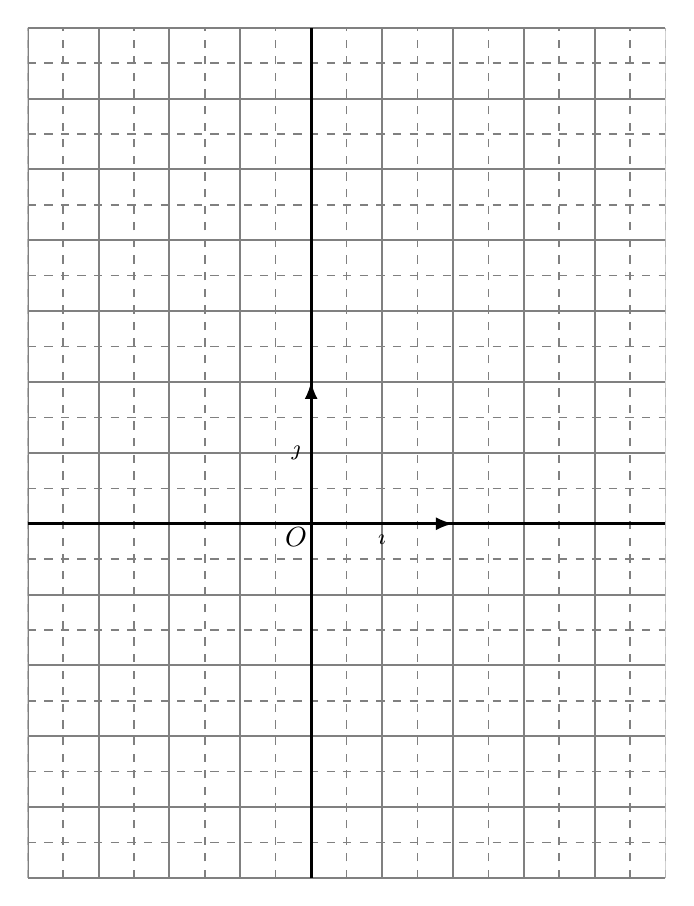
\begin{tikzpicture}[>=latex,scale=0.9,x=2cm,y=2cm]
                    \clip (-2,-2.5) rectangle (2.5,3.5);
                    \draw[color=white,line width=1pt] plot[domain=-1.5:2,samples=200] (\x,{(-\x-1)*(2*\x-3)});
                    \draw[help lines,dashed,line width=0.5pt] (-2,-2.5) grid[step=0.25] (2.5,3.5);
                    \draw[help lines,line width=0.7pt] (-2,-2.5) grid[step=0.5] (2.5,3.5);
                    \draw[-,line width=1pt] (-2,0) -- (2.5,0); \draw[-,line width=1pt] (0,-2.5) -- (0,3.5);
                    \coordinate (O) at (0,0); \draw (O) node[below left = -2pt] {$O$};
                    \coordinate (I) at (1,0); \draw[->,line width=1.1pt] (O) -- (I) node[midway,below] {\footnotesize $\vect\imath$};
                    \coordinate (J) at (0,1); \draw[->,line width=1.1pt] (O) -- (J) node[midway,left] {\footnotesize $\vect\jmath$};
                \end{tikzpicture}
            \end{center}
        \item Résoudre graphiquement l'équation $f(x) = 0$.
        \item Résoudre graphiquement l'inéquation $f(x) > 0$.
        \item Démontrer que pour tout $x \in \R$, $f(x) = (-x -1)(2x - 3)$.
        \item Par le calcul, résoudre $f(x) = 0$.
        \item À l'aide du signe de $-x-1$ et de $2x - 3$, compléter le tableau de signes de la fonction $f$. \bigskip

            \begin{center}
                \begin{tikzpicture}
                    \tkzTabInit[nocadre,espcl=3]{{$x$}/1,{}/1,{}/1,{}/1.25}{$-\infty$,,,,$+\infty$}
                    \tkzTabLine{,,,}
                    \tkzTabLine{,,,}
                    \tkzTabLine{,,,}
                \end{tikzpicture}
            \end{center}
\end{enumerate}



\end{document} 